\documentclass[tikz,border=2pt]{standalone}
\usepackage{amsmath}
\usepackage{pgfplots}
\pgfplotsset{compat=1.18}
\usetikzlibrary{arrows.meta}
\begin{document}
% Assignment stores a value, not a formula: after a <- 1; b <- 10 * a; a <- 100,
% a holds 100 but b still holds 10.
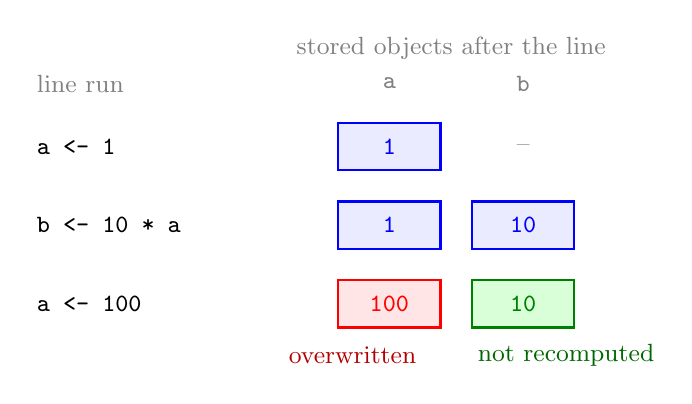
\begin{tikzpicture}[font=\small, >={Latex[length=2mm]},
  code/.style={anchor=west, font=\small\ttfamily},
  obj/.style={draw, thick, minimum width=13mm, minimum height=6mm, inner sep=1pt, font=\small\ttfamily}]
  \node[anchor=west, gray] at (0,3) {line run};
  \node[gray] at (4.6,3) {\texttt{a}};
  \node[gray] at (6.3,3) {\texttt{b}};
  \node[anchor=west, gray] at (3.3,3.45) {stored objects after the line};
  % row 1
  \node[code] at (0,2.2) {a <- 1};
  \node[obj, blue, fill=blue!8] at (4.6,2.2) {1};
  \node[gray] at (6.3,2.2) {--};
  % row 2
  \node[code] at (0,1.2) {b <- 10 * a};
  \node[obj, blue, fill=blue!8] at (4.6,1.2) {1};
  \node[obj, blue, fill=blue!8] at (6.3,1.2) {10};
  % row 3
  \node[code] at (0,0.2) {a <- 100};
  \node[obj, red, fill=red!10] at (4.6,0.2) {100};
  \node[obj, green!50!black, fill=green!15] at (6.3,0.2) {10};
  \node[anchor=west, red!70!black] at (3.2,-0.45) {overwritten};
  \node[anchor=west, green!40!black] at (5.6,-0.45) {not recomputed};
\end{tikzpicture}
\end{document}
